%----------------------------------------------------------------------------
\chapter{Monitor forráskód generátor}
%----------------------------------------------------------------------------

%----------------------------------------------------------------------------
\section{A monitor interfészei}
%----------------------------------------------------------------------------

A monitorozás alatt lévő rendszer egy közös interfészen keresztül kommunikál a monitorral. Az interfész Java implementációja a 19. ábrán tekinthető meg. A monitor azt vizsgálja, hogy a rendszer a scenario szerint működik-e.

Monitor interfész:
\begin{itemize}
    \item update(): a monitorban tárolt rendszer állapotát frissíti a paraméterben kapott üzenet alapján.
    \item goodStateReached(): a rendszer aktuális állapotát jelzi.
    \item requirementSatisfied(): jelzi hogy a rendszer megfelel-e a követelménynek
    \item errorDetected(): detektált hiba jelzésére szolgál
\end{itemize}

Az update() függvényt a rendszer hívja, hogy továbbítsa az üzenetet a monitornak. Paraméterként az üzenet küldőjét (sender), fogadóját (receiver), üzenet nevét (messageType) és az üzenet paramétereit várja (parameters). A goodStateReached() függvényt a monitor hívja amikor a rendszer állapota változik. Ha a rendszer nem elfogadó állapotban van akkor igazat ad vissza, ha pedig nem akkor hamisat. A requirementSatisfied() függvényt is a monitor hívja. Ha a követelménynek megfelelt a rendszer viselkedése akkor igazat ad vissza, amúgy hamisat.

Az üzenetek megfigyeléséhez szükséges segédfüggvényeket a kommunikációs infrastruktúrához kézzel kell megírni. Ezek a monitort az update() függvényen keresztül hívják.

\begin{figure}[!ht]
    \centering
    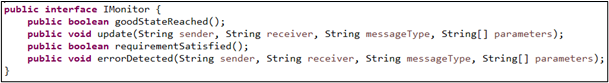
\includegraphics[width=150mm, keepaspectratio]{figures/17abra.png}
    \caption{Monitor interfész Java implementációja.}
\end{figure}

Az időzitő komponenshez tartozik egy időzitő interfész amin keresztül elérhető a komponens. Ezen az interfészen keresztül lehet az óraváltozokat lekérdezni vagy nullázni. Két függvénye van:
\begin{itemize}
    \item getClockVariable(String name): óraváltozó lekérdezése név alapján
    \item resetClockVariable(String name): óraváltozó nullázása név alapján
\end{itemize}

%----------------------------------------------------------------------------
\section{A monitor forráskód megvalósítása}
%----------------------------------------------------------------------------
A generált forráskód struktúrája egy statikus és egy dinamikus részből áll.
A statikus részbe az időzitett automata java osztályai kerülnek:
\begin{itemize}
    \item State: egy állapotot leíró osztály
    \item Transition: egy élet reprezentáló osztály
    \item Automaton: egy automatát megvalósitó osztály
\end{itemize}

A monitor interfész és a monitor java osztálya is ebbe a részbe tartozik.

A dinamikus részben található a Specification Java osztály, ami a scenario alapján generált automata forráskódját tartalmazza. Ezt a 20. ábra mutatja be. A dinamikus rész pirosan van bekeretezve és a statikus rész pedig feketén.

\begin{figure}[!ht]
    \centering
    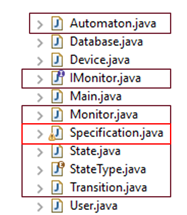
\includegraphics[width=150mm, keepaspectratio]{figures/18abra.png}
    \caption{A monitor forráskódjának struktúrája.}
\end{figure}

A szükséges forráskódok generálásához az Xtend technológiát használtam. Az előző fejezetben ismertetett generátort kiegészítettem egy Monitor Java osztállyal, ami a monitor forráskódjának implementációját tartalmazza.

%----------------------------------------------------------------------------
\section{Minta példa}
%----------------------------------------------------------------------------

A 21. ábrán látható egy scenario követelmény, amit egy példa okos telefon működésére specifikáltunk. Az okos telefonon van egy zene lejátszási lista generáló alkalmazás. A követelményben azt várjuk el, hogy ha a felhasználó megnyitja az alkalmazást akkor a belső kamera készít az arcáról egy képet. A kép alapján eldönti, hogy milyen a felhasználó kedve és az alapján előállít egy zene lejátszási listát.

A 23. ábrán látható az okos telefon és a monitor közti kapcsolat megvalósítása Java kódban és a 22. ábrán pedig egy monitor kimenet. A monitor a rendszertől kapott üzenetek alapján jelzi, hogy a követelmény alapján mi a rendszer állapota.

\begin{figure}[!ht]
    \centering
    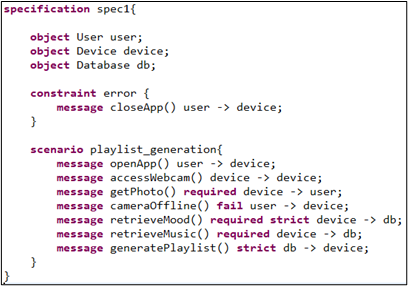
\includegraphics[width=150mm, keepaspectratio]{figures/19abra.png}
    \caption{Okos telefon működésére megadott scenario követelmény.}
\end{figure}

\begin{figure}[!ht]
    \centering
    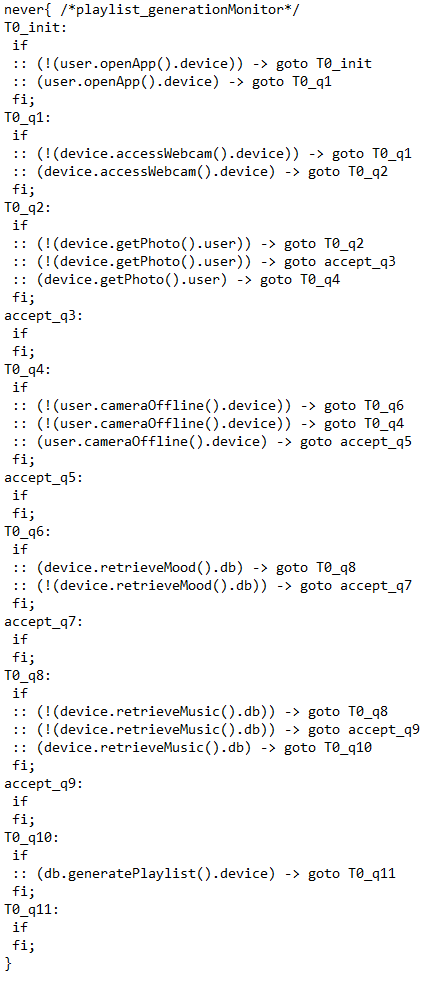
\includegraphics[width=150mm, keepaspectratio]{figures/20abra.png}
    \caption{Generált automata Never claim formátumba.}
\end{figure}

\begin{figure}[!ht]
    \centering
    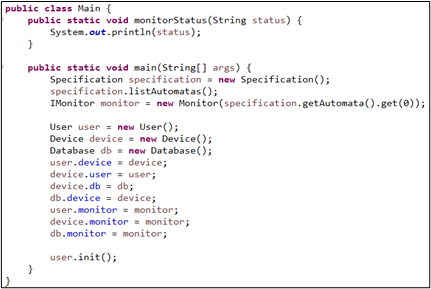
\includegraphics[width=150mm, keepaspectratio]{figures/21abra.png}
    \caption{Az okos telefon és hozzá tartozó monitor összecsatolásának Java implementációja.}
\end{figure}

\begin{figure}[!ht]
    \centering
    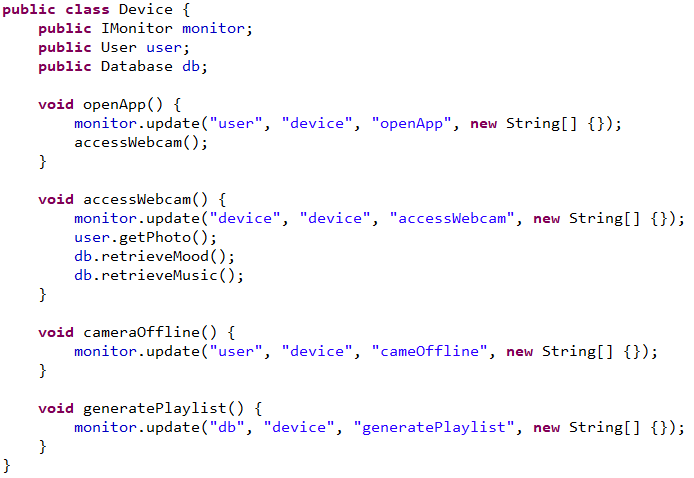
\includegraphics[width=150mm, keepaspectratio]{figures/22abra.png}
    \caption{Az okos telefon Java osztálya.}
\end{figure}

A 24. ábrán látható az okos telefon Java osztálya. Megtekinthető a monitor és az eszköz közti kommunikáció megvalósítása is.

\begin{figure}[!ht]
    \centering
    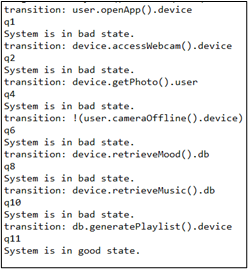
\includegraphics[width=150mm, keepaspectratio]{figures/23abra.png}
    \caption{Monitor kimenete a rendszer működésének egyes fázisaiban.}
\end{figure}
A 25. ábrán látszik, hogy a rendszer a működése elején nem felelt meg a monitor követelményének. Amikor a működése végére ért akkor a monitor jelezte, hogy a követelmény teljesült a „Good state” üzenettel. A mintához tartozó Specification osztály a függelékben található. A generált automatát a konstruktorában állítja elő.